\documentclass[
    linespread = 1.25
]{ctexart}
\pagestyle{plain}
\ctexset{
    section/format = \Large\bfseries\raggedright,
    section/number = {\chinese{section}、},
    section/aftername = {\enskip},
    abstractname = {\zihao{-2}摘\quad 要}
}

\usepackage[a4paper, lmargin=1in, rmargin=1in, tmargin=1in, bmargin=1in]{geometry}
\usepackage{amsmath}
\usepackage{booktabs}
\usepackage{graphicx}
\graphicspath{ {./fig} }

\usepackage{listings}
\usepackage{color}

\definecolor{dkgreen}{rgb}{0,0.6,0}
\definecolor{gray}{rgb}{0.5,0.5,0.5}
\definecolor{mauve}{rgb}{0.58,0,0.82}

\lstset{
  frame=tb,
  language=Python,
  aboveskip=3mm,
  belowskip=3mm,
  showstringspaces=false,
  columns=flexible,
  basicstyle={\small\ttfamily},
  numbers=left,
  numberstyle=\tiny\color{gray},
  keywordstyle=\color{blue},
  commentstyle=\color{dkgreen},
  stringstyle=\color{mauve},
  breaklines=true,
  breakatwhitespace=true,
  tabsize=2
}

\usepackage[hidelinks]{hyperref}
\usepackage{caption}
\usepackage{subcaption}
\usepackage{siunitx}
\usepackage{algorithm2e}
\SetAlgoInsideSkip{bigskip}
\SetAlgorithmName{算法}{算法}{算法}
\RestyleAlgo{ruled}
\usepackage{multicol}
\usepackage{longtable}
\usepackage{tablefootnote}

\title{\zihao{2}\textbf{模式识别实验二}}
\author{\zihao{4}210810508 - 彭珂\\\texttt{1094451830@qq.com}
\and \zihao{4}210810510 - 刘炎培\\\texttt{liu\_yanpei@outlook.com}
}
\date{}

\begin{document}

\maketitle
\tableofcontents
\newpage

\section{数据预处理与可视化}

\subsection{数据介绍}

本实验的数据来源于Mathlib4开源项目\cite{mathlib4},该项目是一个数学证明库,其中包含了大量的数学定理和证明。在Mathlib4中,相关的数学定理和证明被组织成了单个lean4文件,每个lean4文件中包含了一个或多个数学定理和证明。在本实验中,我们将lean4文件看作是一个节点,节点之间的依赖关系看作是一条有向边,这样我们就可以将Mathlib4中的数学定理和证明组织成一个有向图。

\subsection{数据预处理}

Mathlib4中不仅有数学定理的证明,还包括一些lean4的库文件、编译脚本、证明策略等等。在本实验中,我们筛选出了数学定理和证明,而去除了其他文件。然后进行依赖的提取。

为了快速地得到Mathlib4中数学概念的大致依赖关系,我们把每个lean4文件中直接使用import关键字引入的其他lean4文件看作是该文件的一个依赖,而没有使用编译器前端或者lsp等进行依赖分析。但实际上,由于lean4灵活的命名空间,lean4文件之间的依赖关系可能会比我们所统计的要复杂。另一方面,单个lean4文件也可能包含相当多的数学定理和证明,这具体取决于代码贡献者是否严格遵循Mathlib4的编程规范以及仓库管理者是否对代码贡献者的代码进行了严格地审核。因此,我们的数据只能作为Mathlib4中数学定理和证明的一个大致依赖关系的参考。

按照上面的方法,我们把Mathlib4中的文件的依赖关系提取出来之后,共有4910个节点和13858条边,我们把数据保存为一个json文件,以便之后使用。

\subsection{数据可视化}

把上文中提取出的数据进行可视化,我们可以得到Mathlib4中各个学科的依赖图。图中的每个节点代表一个lean4文件,节点之间的边代表依赖关系,节点的颜色取决于其所在的子学科,边的颜色与被依赖的节点相同。下图\ref{fig:dependency}展示了Mathlib4中的各个子学科的依赖关系。

\begin{figure}[H]
    \centering
    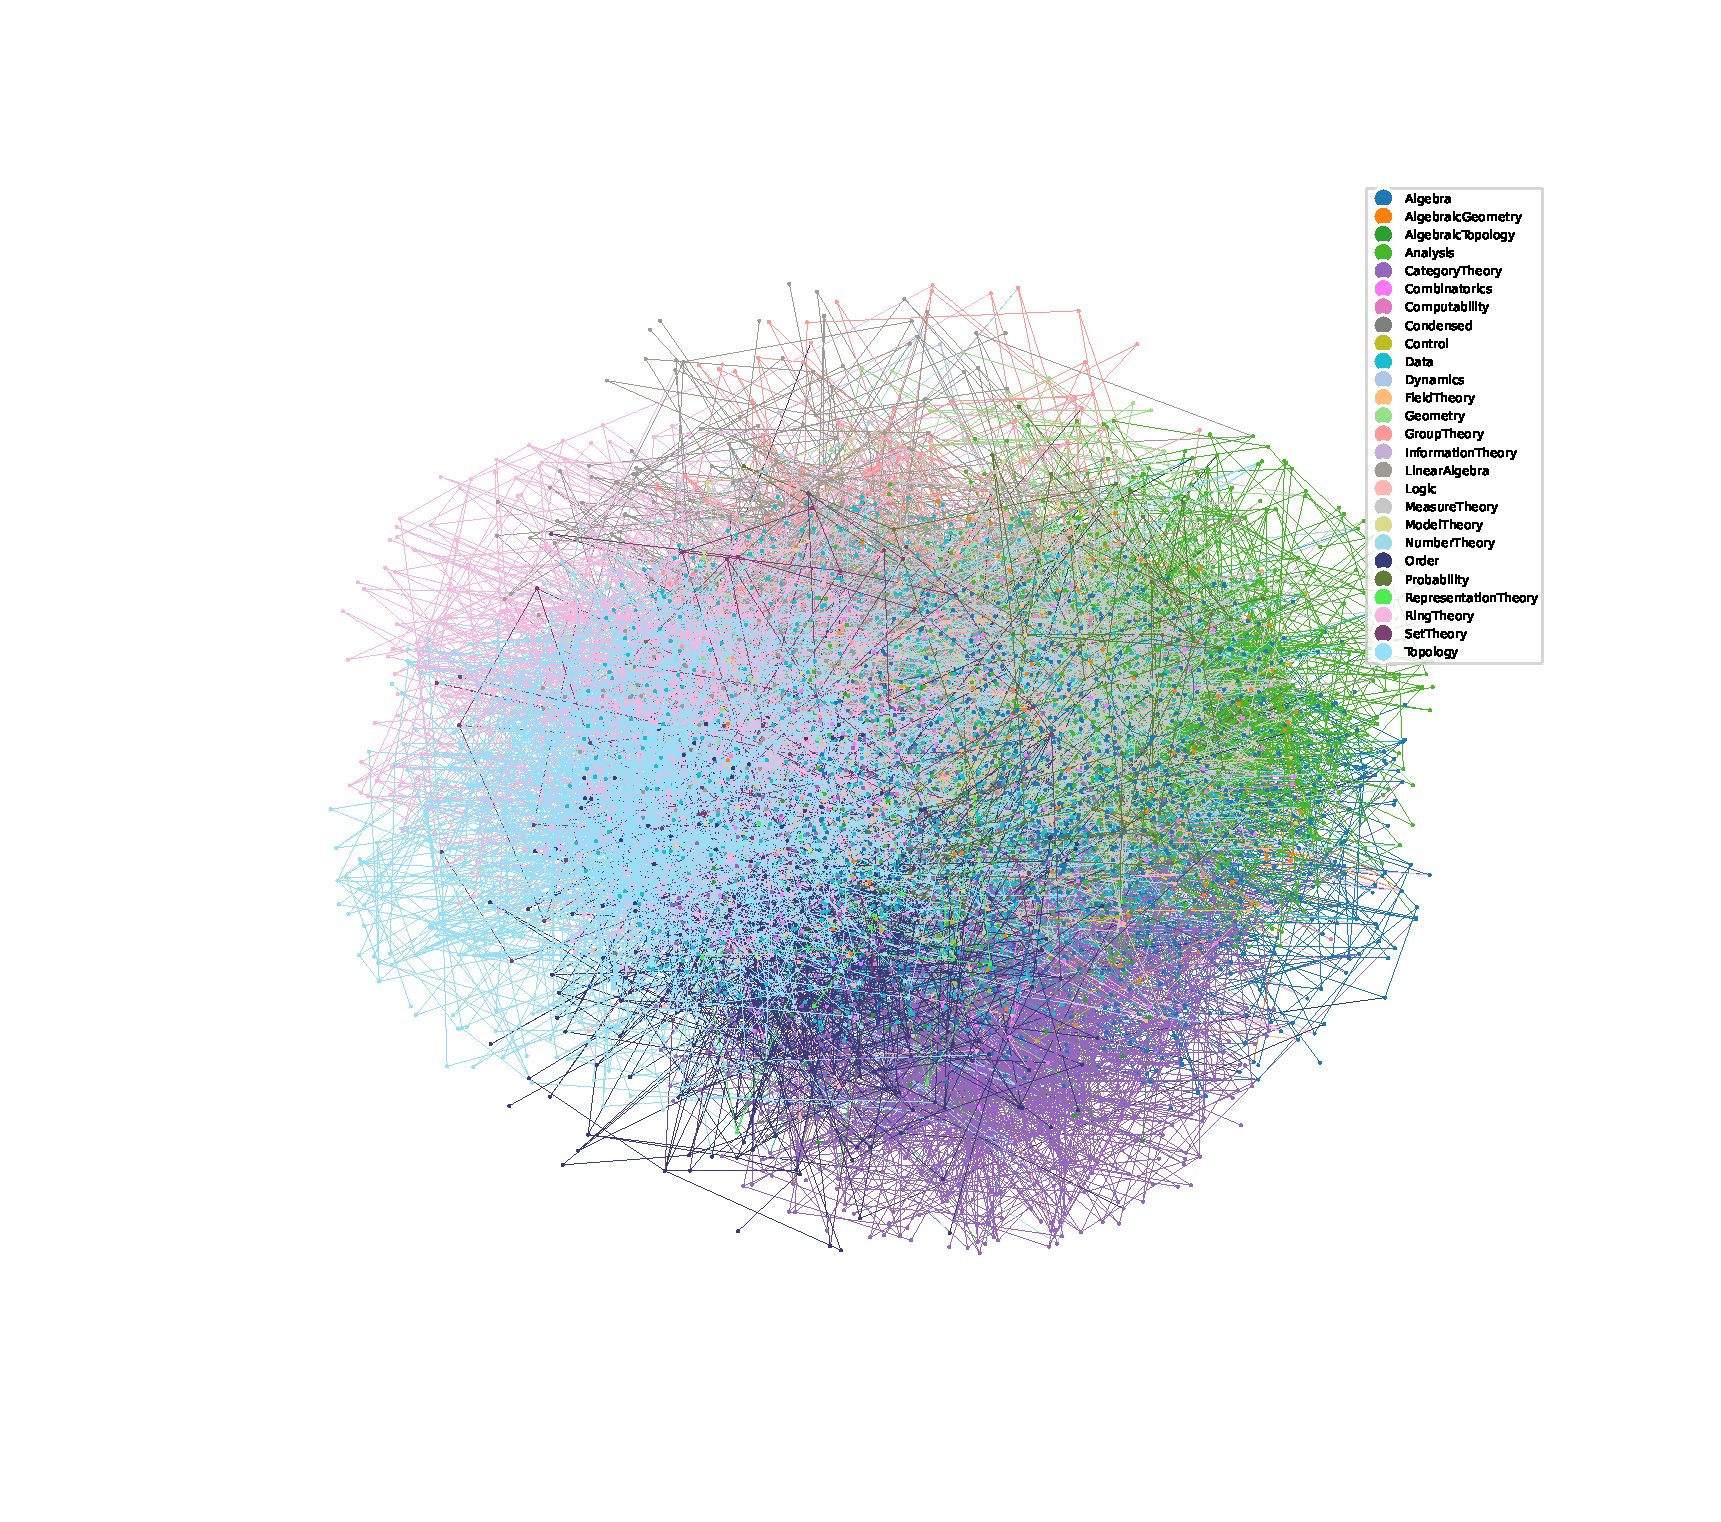
\includegraphics[width=1.0\textwidth]{../img/data.pdf}
    \caption{Dependency graph of Mathlib4}
    \label{fig:dependency}
\end{figure}


\section{社群识别与聚类}

\subsection{数据分析}

在进行社群识别之前,我们首先对数据进行一个粗略的分析。我们统计了每个子学科的节点数、任一端点位于学科内的边的数量、边的两个端点均属于该学科的边的数量及比例以及学科节点占总节点的比例。统计结果如表\ref{tab:Ratio}所示。

\begin{table}[H]
\centering
\begin{tabular}{llllll}
    \toprule
    Subject & Nodes & Edges & EdgesInSameSubject & EdgesRatio & NodesRatio\\ 
    \midrule
    Algebra & 894 & 6058 & 1939 & 0.32 & 0.18\\
    AlgebraicGeometry & 70 & 303 & 100 & 0.33 & 0.01\\
    AlgebraicTopology & 43 & 171 & 53 & 0.31 & 0.01\\
    Analysis & 488 & 2708 & 972 & 0.36 & 0.10\\
    CategoryTheory & 591 & 3351 & 1403 & 0.42 & 0.12\\
    Combinatorics & 107 & 429 & 112 & 0.26 & 0.02\\
    Computability & 18 & 66 & 15 & 0.23 & 0.00\\
    Condensed & 25 & 121 & 33 & 0.27 & 0.01\\
    Control & 25 & 112 & 28 & 0.25 & 0.01\\
    Data & 576 & 3144 & 801 & 0.25 & 0.12\\
    Dynamics & 23 & 95 & 16 & 0.17 & 0.00\\
    FieldTheory & 52 & 292 & 71 & 0.24 & 0.01\\
    Geometry & 80 & 311 & 109 & 0.35 & 0.02\\
    GroupTheory & 119 & 649 & 157 & 0.24 & 0.02\\
    InformationTheory & 1 & 1 & 0 & 0.00 & 0.00\\
    LinearAlgebra & 233 & 1411 & 402 & 0.28 & 0.05\\
    Logic & 50 & 383 & 55 & 0.14 & 0.01\\
    MeasureTheory & 196 & 1001 & 350 & 0.35 & 0.04\\
    ModelTheory & 29 & 118 & 41 & 0.35 & 0.01\\
    NumberTheory & 149 & 643 & 168 & 0.26 & 0.03\\
    Order & 209 & 1281 & 331 & 0.26 & 0.04\\
    Probability & 61 & 221 & 85 & 0.38 & 0.01\\
    RepresentationTheory & 15 & 83 & 18 & 0.22 & 0.00\\
    RingTheory & 368 & 2169 & 638 & 0.29 & 0.07\\
    SetTheory & 46 & 216 & 55 & 0.25 & 0.01\\
    Topology& 442 & 2379 & 820 & 0.34 & 0.09\\
    \bottomrule
\end{tabular}
\caption{Some basic data for each subject}
\label{tab:Ratio}
\end{table}

我们知道,对于一张随机图,当NodeRatio较小时,EdgesRatio应大致为NodesRatio的一半,而实际上EdgesRatio远大于NodesRatio的一半,说明这张图中确实存在社群结构,且该结构一定程度上被学科分类所反映。可以算出,按学科进行分类的modularity为0.527, 说明学科分类对于该图的社群结构有着一定的解释力。

我们下面尝试使用谱聚类的方法来找到这些社群。
我们使用sklearn.cluster中的SpectralClustering来进行谱聚类,我们将谱聚类的结果与学科分类进行比较,以此来验证该图中的社群是否与按学科划分的社群一致,当然谱聚类本身对社群的划分效果也要做衡量,为此选用adjusted rand score, normalized mutual info score和modularity来作为聚类效果的评价指标。考虑到我们一共有26个子学科,虽然不是每一个学科都很好的形成一个极大的社群,但是大致地将聚类数选成26是合理的。后续我们遍历了2到30的聚类数,最优的聚类数大致在二十多,但实际上,聚类效果的好坏对随机因素相当敏感,选取26作为聚类数的效果并不显著优于或劣于选取21到26之间的其他聚类数。我们对谱聚类的结果进行了可视化,如图\ref{fig:clustering}所示。

\begin{figure}[H]
    \centering
    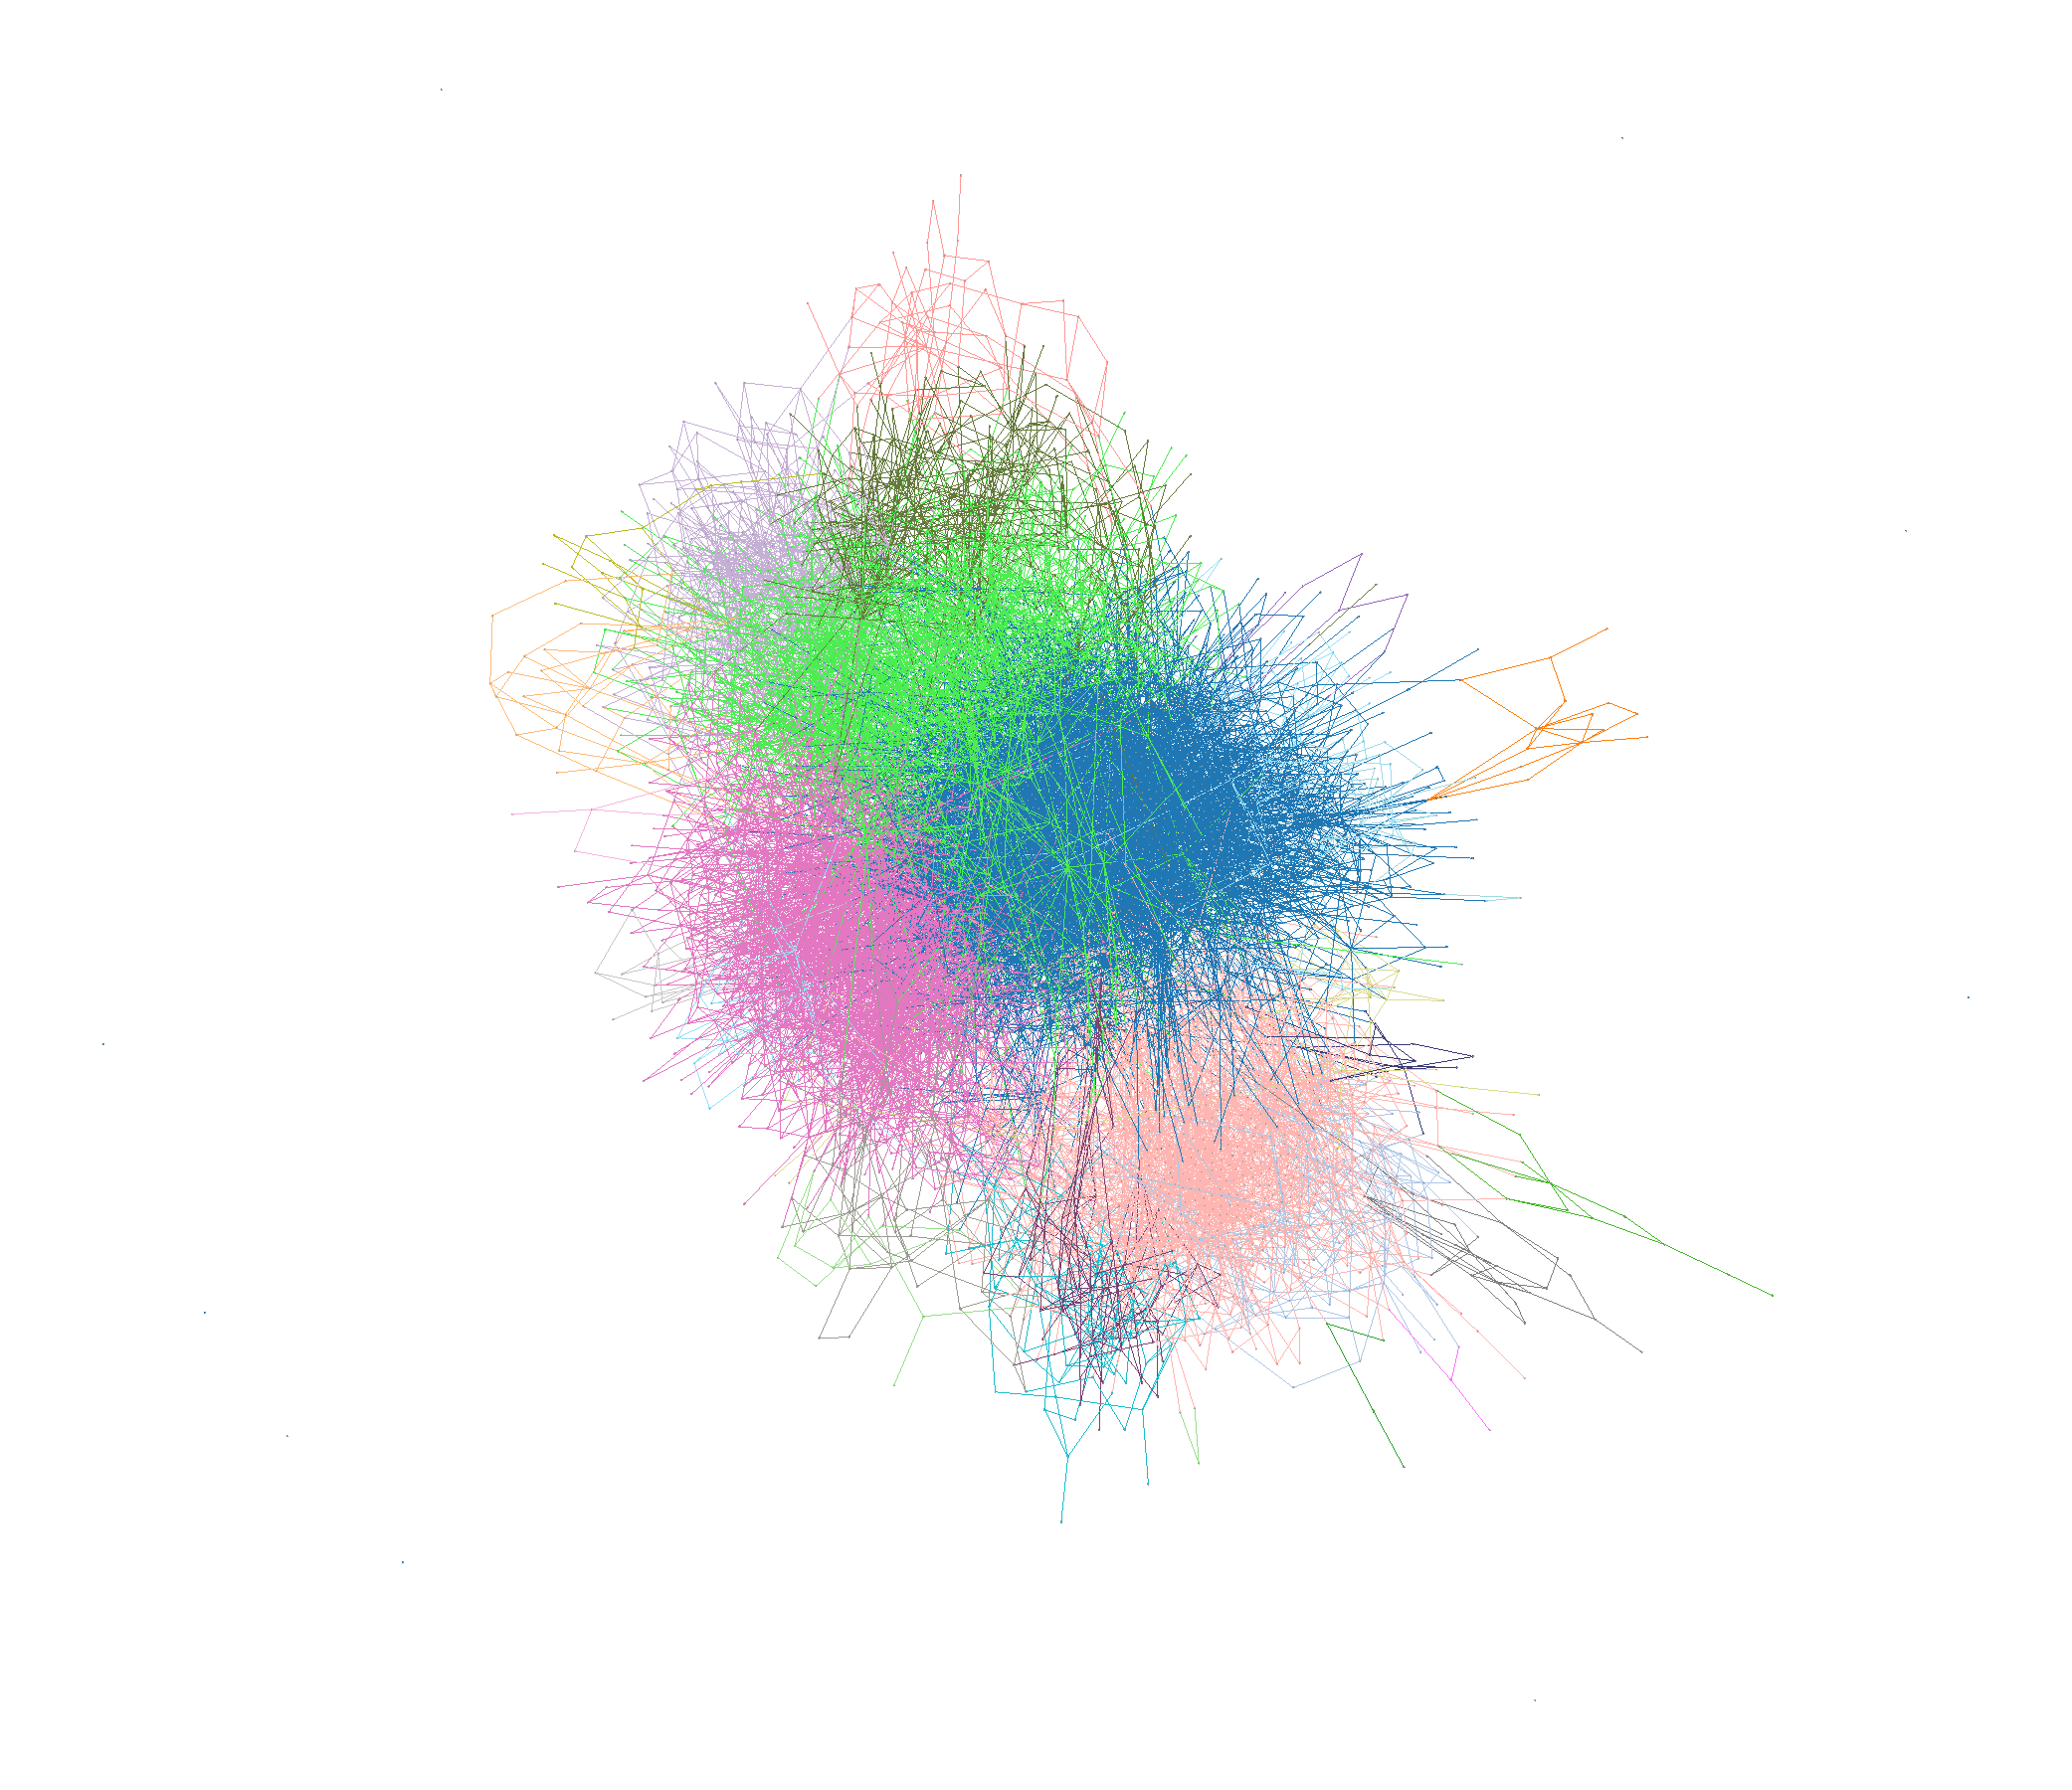
\includegraphics[width=1.0\textwidth]{../img/graph_spectral_cluster.png}
    \caption{Dependency graph of Mathlib4 colored by spectral clustering}
    \label{fig:clustering}
\end{figure}

对应的评价指标如表\ref{tab:score}所示。
\begin{table}[H]
  \centering
  \begin{tabular}{lll}
    \toprule
    ARI & NMI & Modularity\\
    \midrule
    0.260 & 0.475 & 0.614\\
    \bottomrule
  \end{tabular}
  \caption{Evaluation scores of spectral clustering}
  \label{tab:score}
\end{table}

较高的modularity表明聚类效果良好,Mathlib4中的数学概念之间确实有着非常明确的社群结构且该结构被谱聚类很好地捕捉了,但较为一般的ARI和NMI表明谱聚类的结果与学科分类并不完全一致,这是因为Mathlib4中的数学概念之间的依赖关系并不完全由学科决定,而是由数学概念之间的逻辑关系决定的,实际上考虑到使用谱聚类的modularity比按学科分类的modularity要高出9个百分点,我们认为谱聚类的结果与按学科分类的结果不完全一致是符合预期的。

接下来我们使用graph\_tool库中的SBM模型来对Mathlib4进行社群识别。我们分别使用graph\_tool的minimize\_blockmodel\_dl函数和minimize\_nested\_blockmodel\_dl函数来对Mathlib4进行社群识别,得到的结果如图\ref{fig:SBM}和\ref{fig:nest_SBM}所示。

\begin{figure}[H]
    \centering
    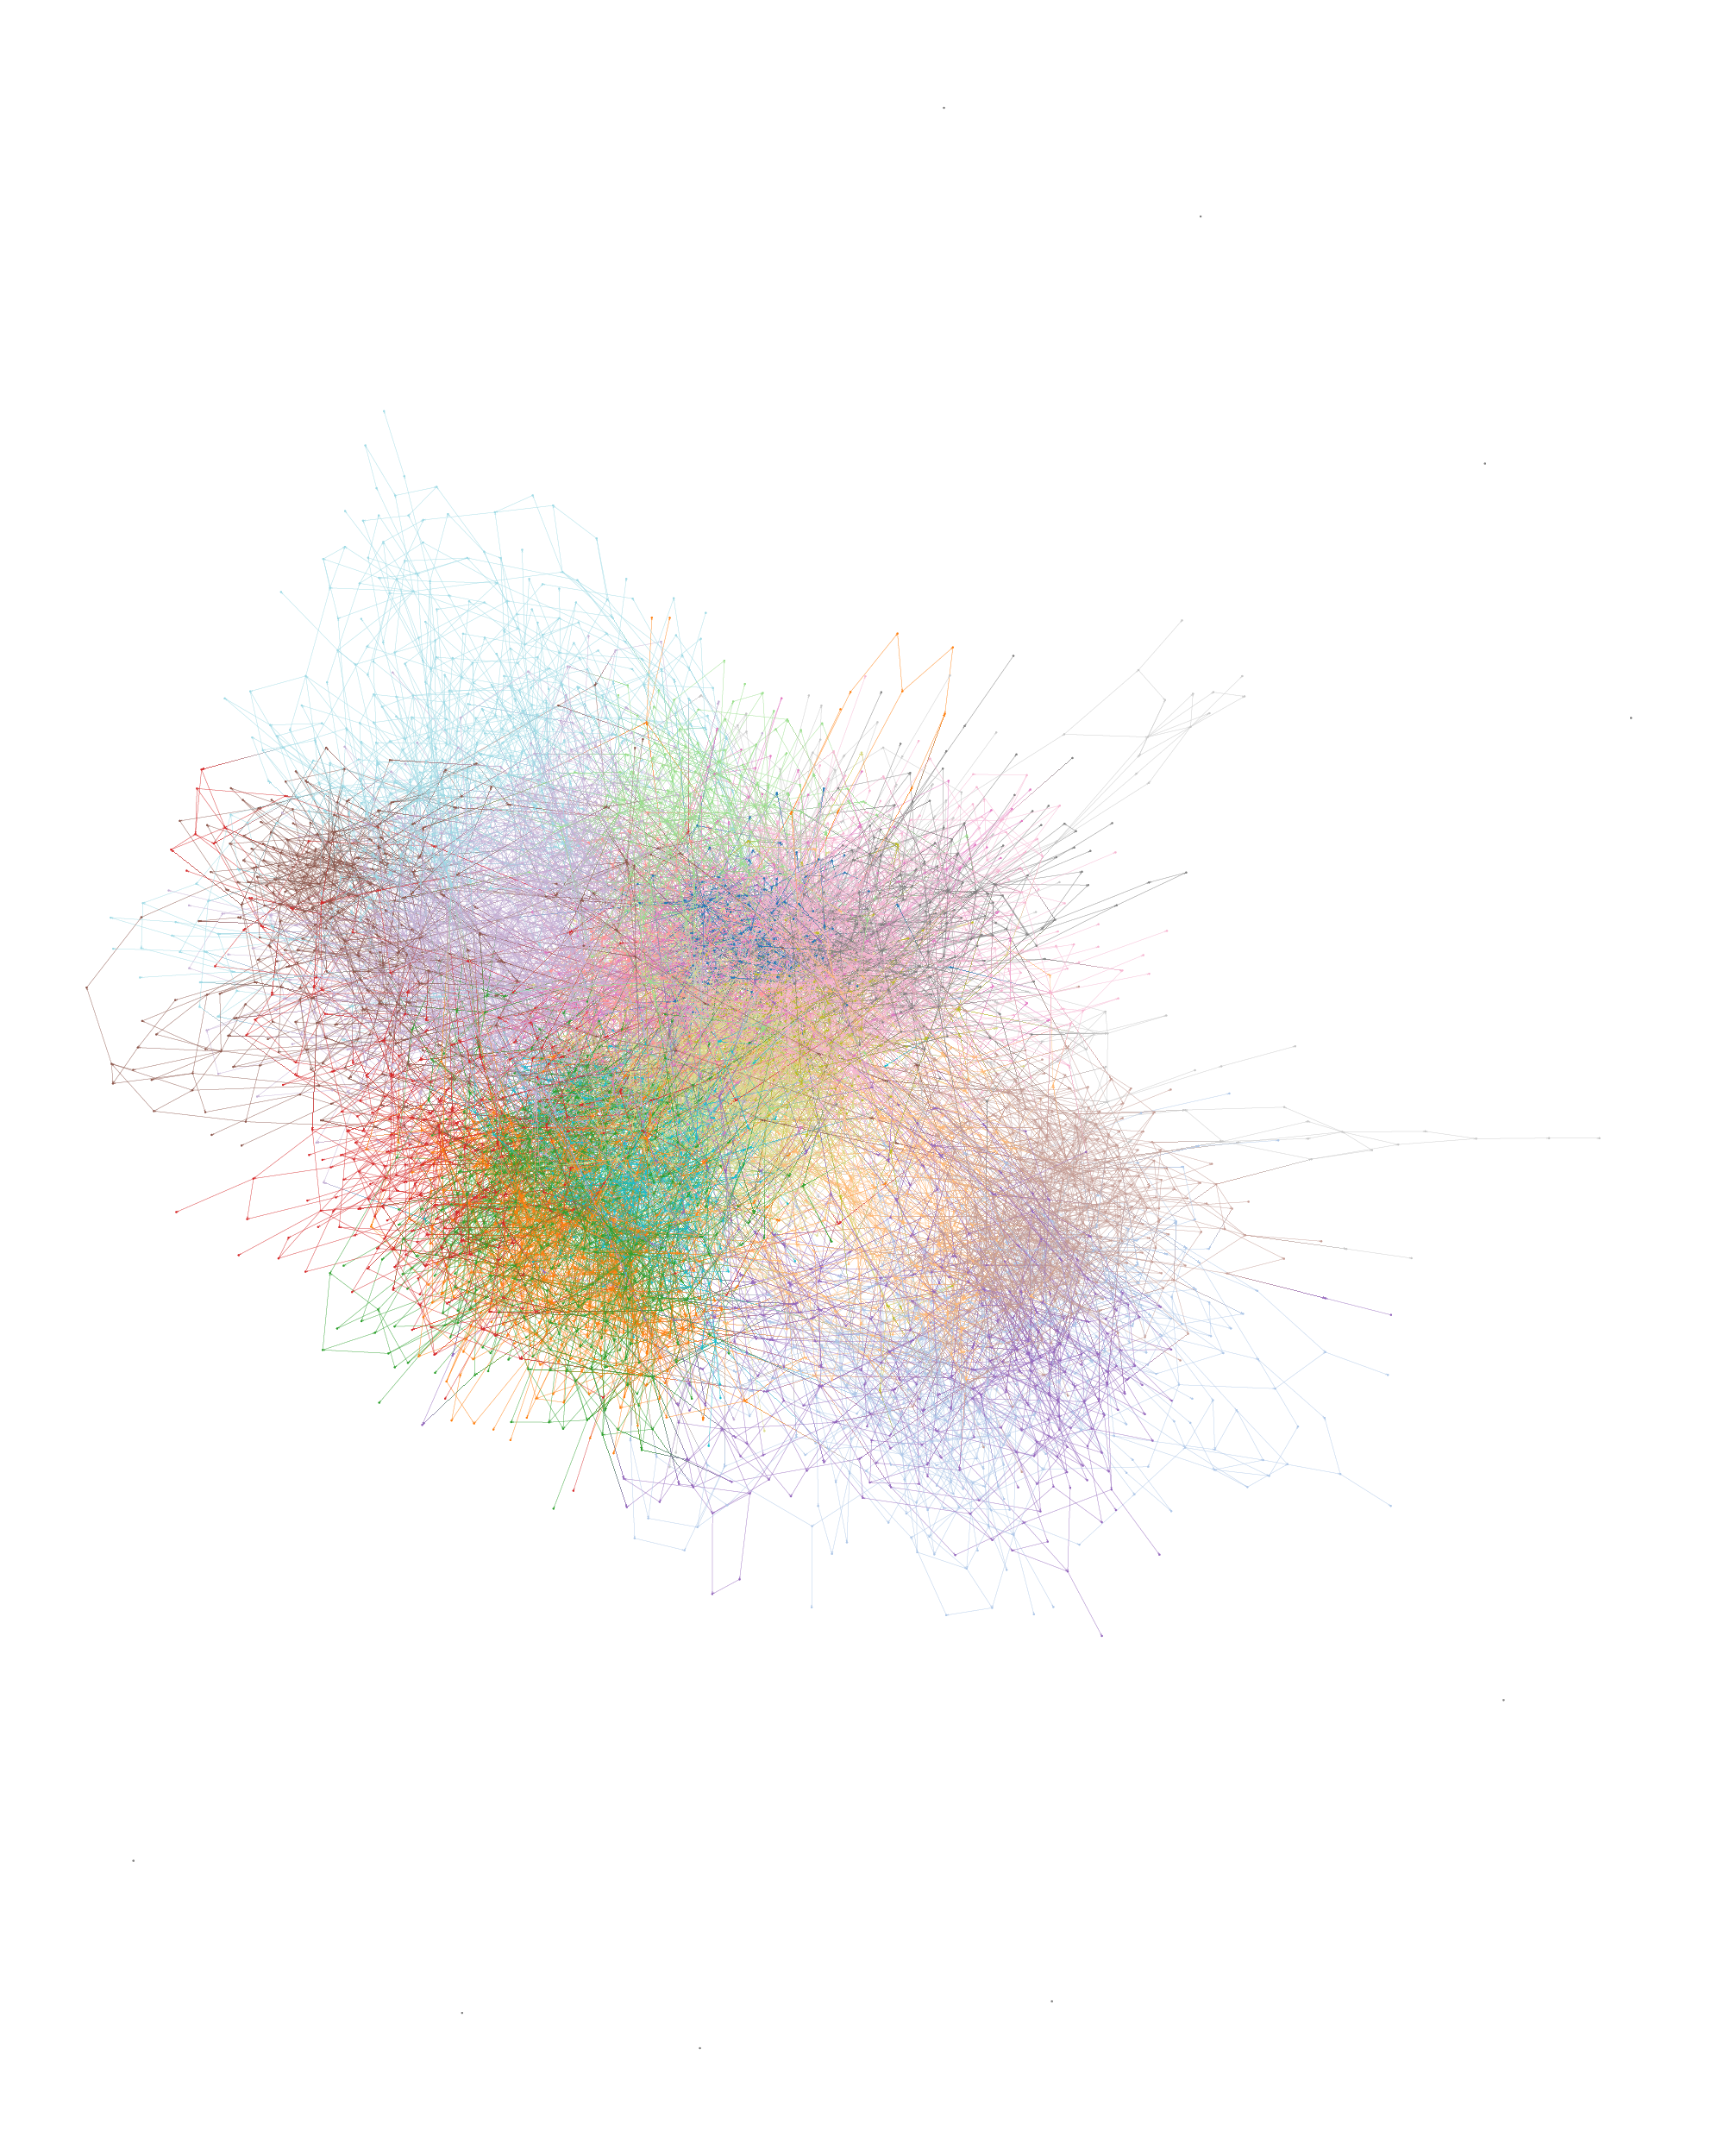
\includegraphics[width=1.0\textwidth]{../img/SBM.png}
    \caption{Dependency graph of Mathlib4 colored by SBM model}
    \label{fig:SBM}
\end{figure}

\begin{figure}[H]
  \centering
  \includegraphics[width=1.0\textwidth]{../img/SBM_nested.png}
  \caption{Dependency graph of Mathlib4 colored by nested SBM model}
  \label{fig:nest_SBM}
\end{figure}

对应的评价指标如表\ref{tab:score2}所示。
\begin{table}[H]
  \centering
  \begin{tabular}{llll}
    \toprule
    Model & ARI & NMI & Modularity\\
    \midrule
    BSM & 0.226 & 0.466 & 0.614\\
    nested BSM & 0.199 & 0.450 & 0.614\\
    \bottomrule
  \end{tabular}
  \caption{Evaluation scores of the SBM model}
  \label{tab:score2}
\end{table}

可以看到,SBM模型的modularity与谱聚类的modularity相同,而ARI和NMI稍低,这说明SBM模型的结果与谱聚类的结果基本一致,但是由于SBM模型的结果是由模型自身决定的,因此与学科分类的结果并不完全一致。






% set figure directory
\graphicspath{{../graph_nn/fig/}}
\section{使用图神经网络进行半监督分类}
在上一节中,我们使用了谱聚类和SBM模型对Mathlib4中的数学定理和证明进行了社群识别,并使用modularity、ARI和NMI指标对得到的社群结果进行了评价。从较低的ARI和NMI指标可以看出,我们社群发现的结果相较于按学科进行划分的结果有明显的差异;而从比学科划分更高的modularity指标来看,有理由认为社群发现的结果相较单纯的学科划分更能体现出数学概念之间的逻辑关系。

尽管谱聚类和SBM模型对于数据的社群发现可能提供了学科划分之外新的视角,但是两种方法作为无监督的学习方法,较低的可解释性和较大的评估难度是其固有的缺陷。

在本节中,我们将以每个节点的学科作为标签,使用图神经网络(GNNs)对Mathlib4中的数学定理和证明进行半监督分类。并将模型在测试集上的表现与按学科分类的真实结果进行对比。

\subsection{\texttt{PyTorch}数据准备}
我们使用\texttt{PyTorch Geometric}库来进行图卷积神经网络(GCNs)的构建和训练。为此,我们需要将Mathlib4中的数据转换为\texttt{PyTorch Geometric}中的\texttt{Data}对象,该对象包含了图的结构信息和节点特征信息。具体来说,包括:
\begin{itemize}
    \item \texttt{x}:节点特征矩阵,每一行代表一个节点的特征向量;
    \item \texttt{edge\_index}:边的索引矩阵,每一列代表一条边的起始节点和终止节点的索引;
    \item \texttt{y}:节点标签向量,每一个元素代表一个节点的标签;
    \item \texttt{train\_mask}:训练集掩码向量,每一个元素代表一个节点是否在训练集中(\texttt{val\_mask}和\texttt{test\_mask}同理)。
\end{itemize}

关于节点特征矩阵\texttt{x},因为我们分类仅仅用到的是图的依赖结构,节点特征并不包含额外的信息,我们该如何初始化节点特征矩阵是一个值得考虑的问题。一个简单的想法可能是赋予每个节点相同的特征向量,如\texttt{x}为全零或全一向量。然而这样的初始化使得模型没有办法学习到有用的信息;回头考虑GCN的结构不难发现,这样的初始化使得模型不能够区分不同的节点。对此,一个简单的改进是将\texttt{x}初始化为单位矩阵。值得注意的是,其他可以考虑的选择包括使用Laplacian矩阵的特征向量作为节点特征,或者使用预训练的embedding作为节点特征。

关于图的边索引矩阵\texttt{edge\_index},我们将Mathlib4中的依赖关系作为无向边处理。为了适应GCN的结构,这一简化处理损失了依赖关系的方向性,尽管在数学证明的范畴下这一简化可能是合理的。然而,可能的改进方向包括使用自然考虑到图的方向性的模型如Graph Attention Networks(GATs)。

关于节点标签向量\texttt{y},我们将每个节点的学科作为标签。由于\texttt{Torch}期望标签是从0开始的整数,我们将学科的字符串标签映射到整数标签。

关于训练-验证-测试集的划分,我们选取三者的比例为$8:1:1$,并使用掩码向量做出标记。

\subsection{构建GCN模型并训练}
我们使用\texttt{PyTorch Geometric}库中的\texttt{GCNConv}层来构建GCN模型。我们的模型初步包括两层GCN层,后接一个ReLU激活函数,最后以类别数大小的线性层输出。我们使用交叉熵损失函数和Adam优化器进行训练,注意到\texttt{Torch}中的交叉熵损失函数会自动将Softmax函数作用于线性输出层。

模型可以调整的超参数包括GCN的层数、隐藏层的维度、学习率、epoch数等。通过观察模型在验证集上的表现,我们调整模型为一层GCN,隐藏层维度为512,学习率为0.01,epoch数为30。模型的训练曲线如图\ref{fig:gcn_train}所示。% loss曲线和accuracy曲线

\begin{figure}[htbp]
    \centering
    \begin{subfigure}{0.48\textwidth}
        \centering
        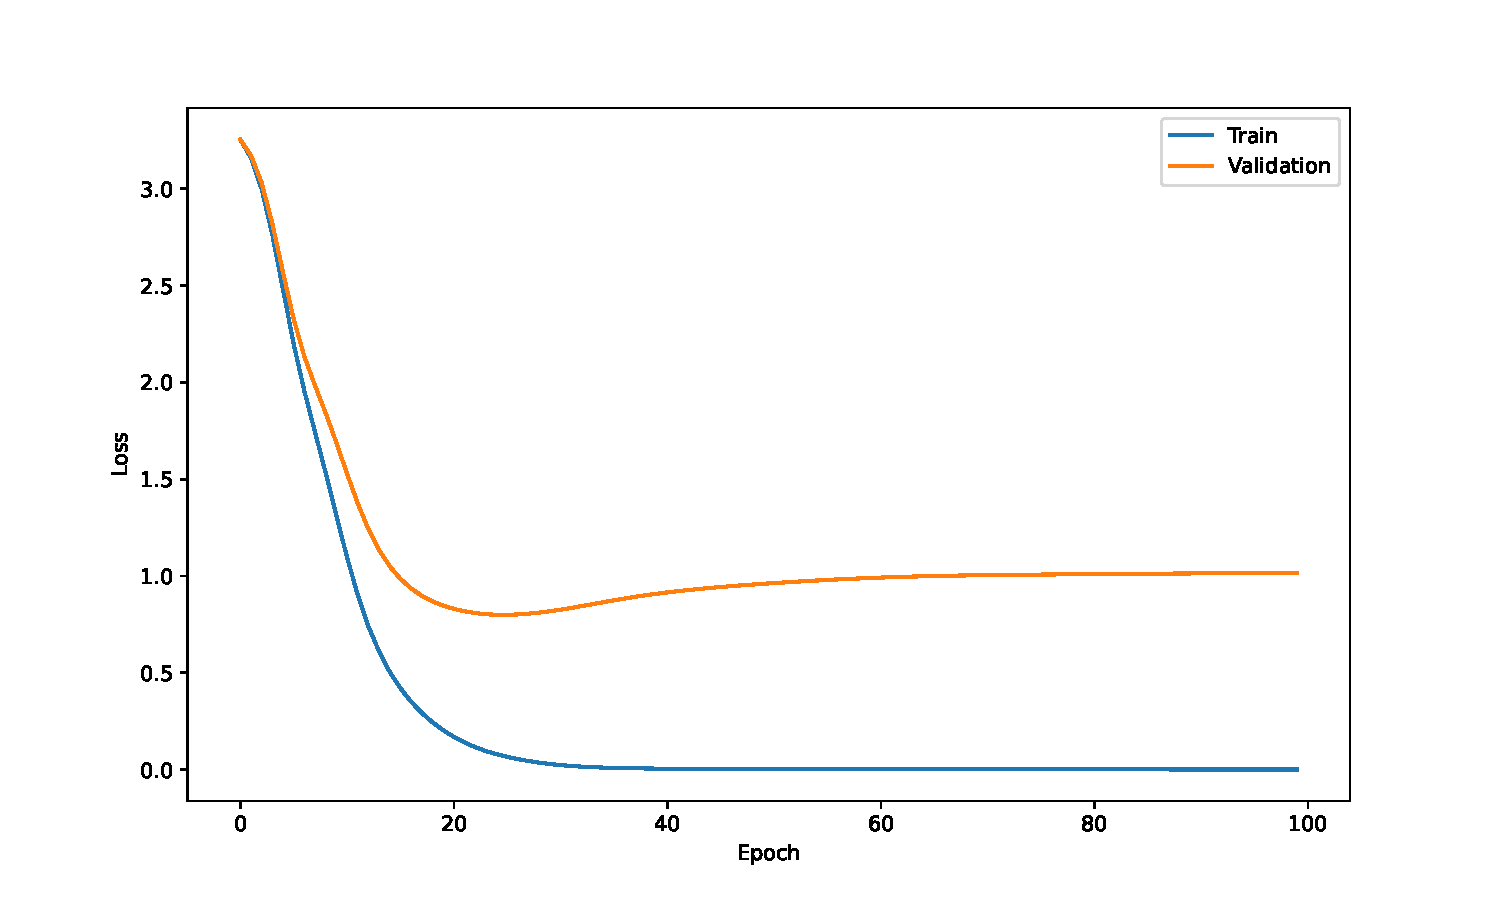
\includegraphics[width=\textwidth]{loss.pdf}
        \caption{Loss曲线}
    \end{subfigure}
    \begin{subfigure}{0.48\textwidth}
        \centering
        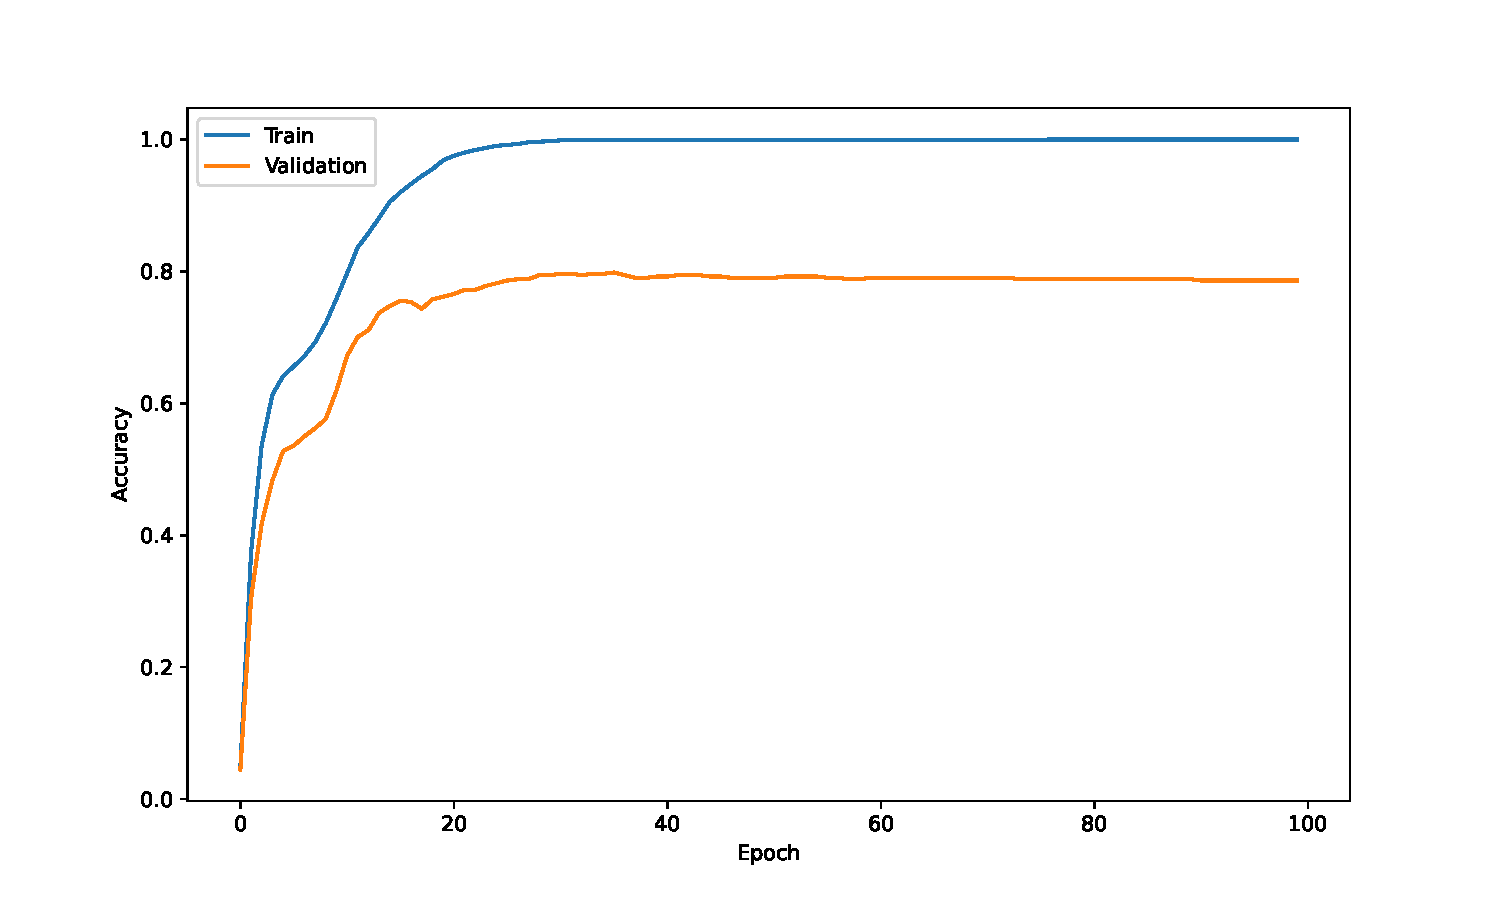
\includegraphics[width=\textwidth]{acc.pdf}
        \caption{Accuracy曲线}
    \end{subfigure}
    \caption{GCN模型训练曲线}
    \label{fig:gcn_train}
\end{figure}

\subsection{模型评估}
我们使用模型在测试集上的准确率和混淆矩阵来评估模型的性能。同时,一个容易想到的Baseline模型是将每个节点的邻居标签众数表决的结果作为预测结果。二者在测试集上的准确率对比如表\ref{tab:gcn_acc}所示。二者的预测结果的混淆矩阵对比如表\ref{tab:gcn_confusion}所示。

\begin{table}[htbp]
    \centering
    \caption{GCN模型和Baseline模型在测试集上的准确率}
    \begin{tabular}{cc}
        \toprule
        模型 & 准确率 \\
        \midrule
        Baseline & 56.01\% \\
        GCN & 76.58\% \\
        \bottomrule
    \end{tabular}
    \label{tab:gcn_acc}
\end{table}

\begin{figure}
    \centering
    \begin{subfigure}{0.48\textwidth}
        \centering
        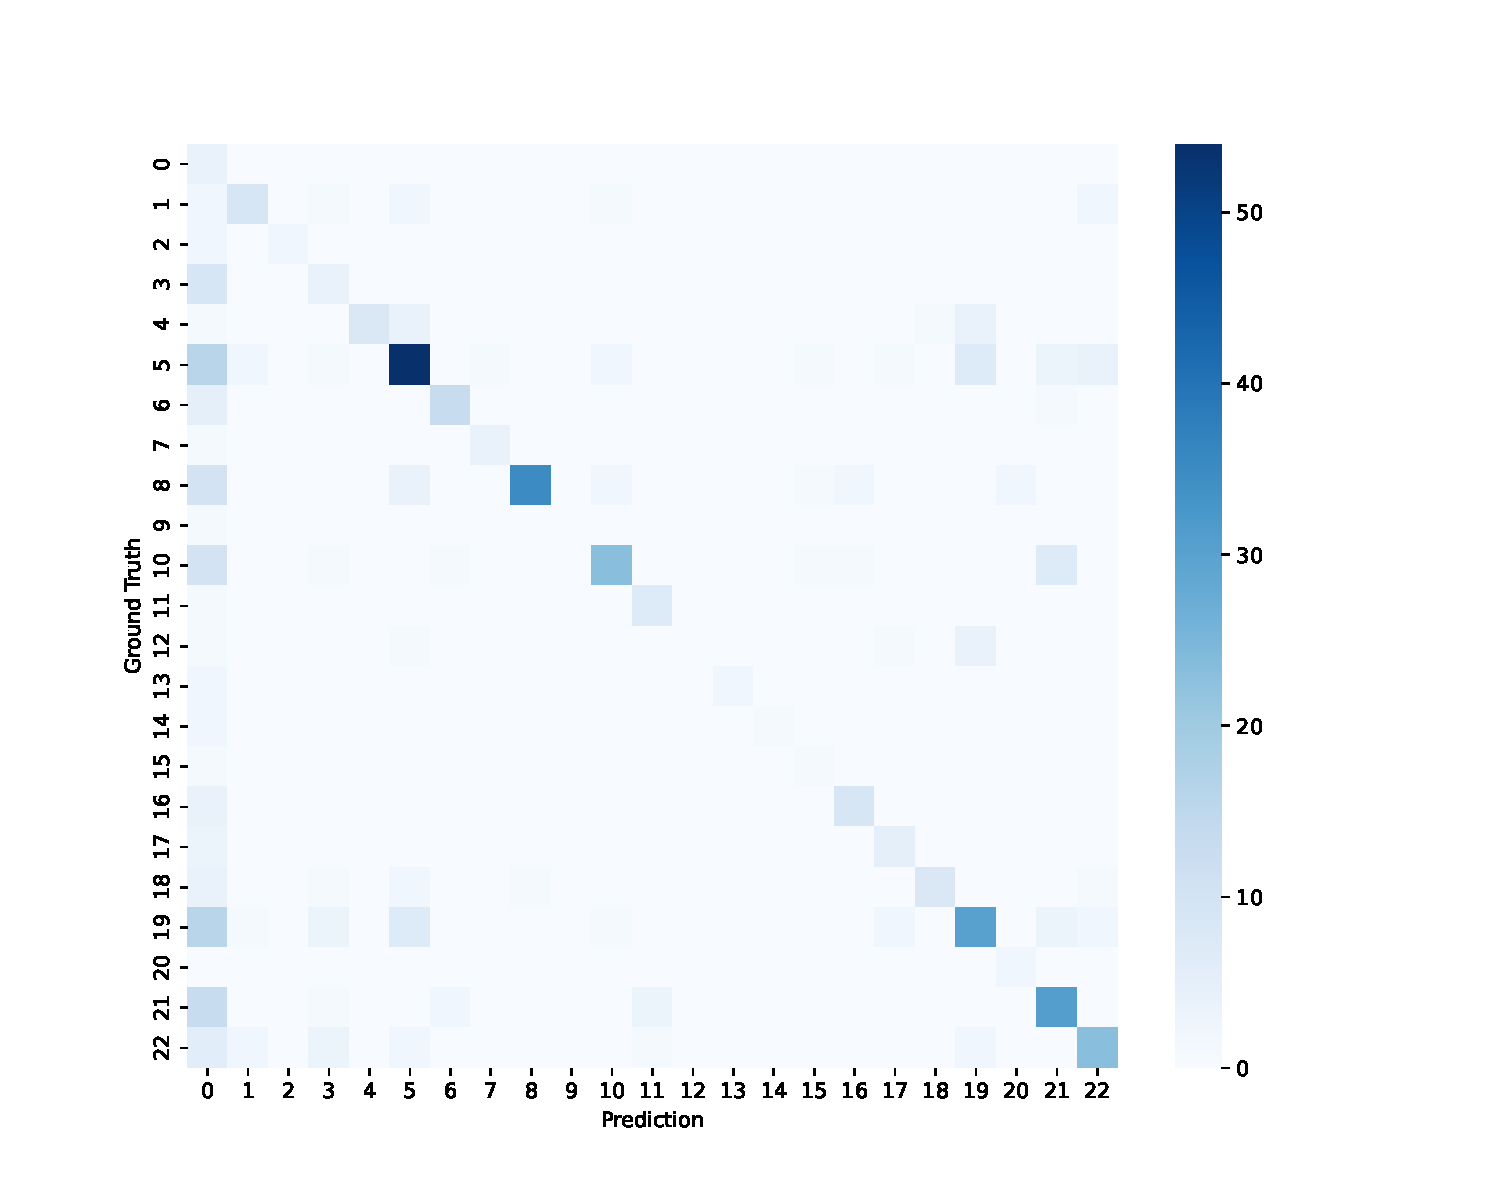
\includegraphics[width=\textwidth]{confusion_matrix_baseline.pdf}
        \caption{Baseline模型}
    \end{subfigure}
    \begin{subfigure}{0.48\textwidth}
        \centering
        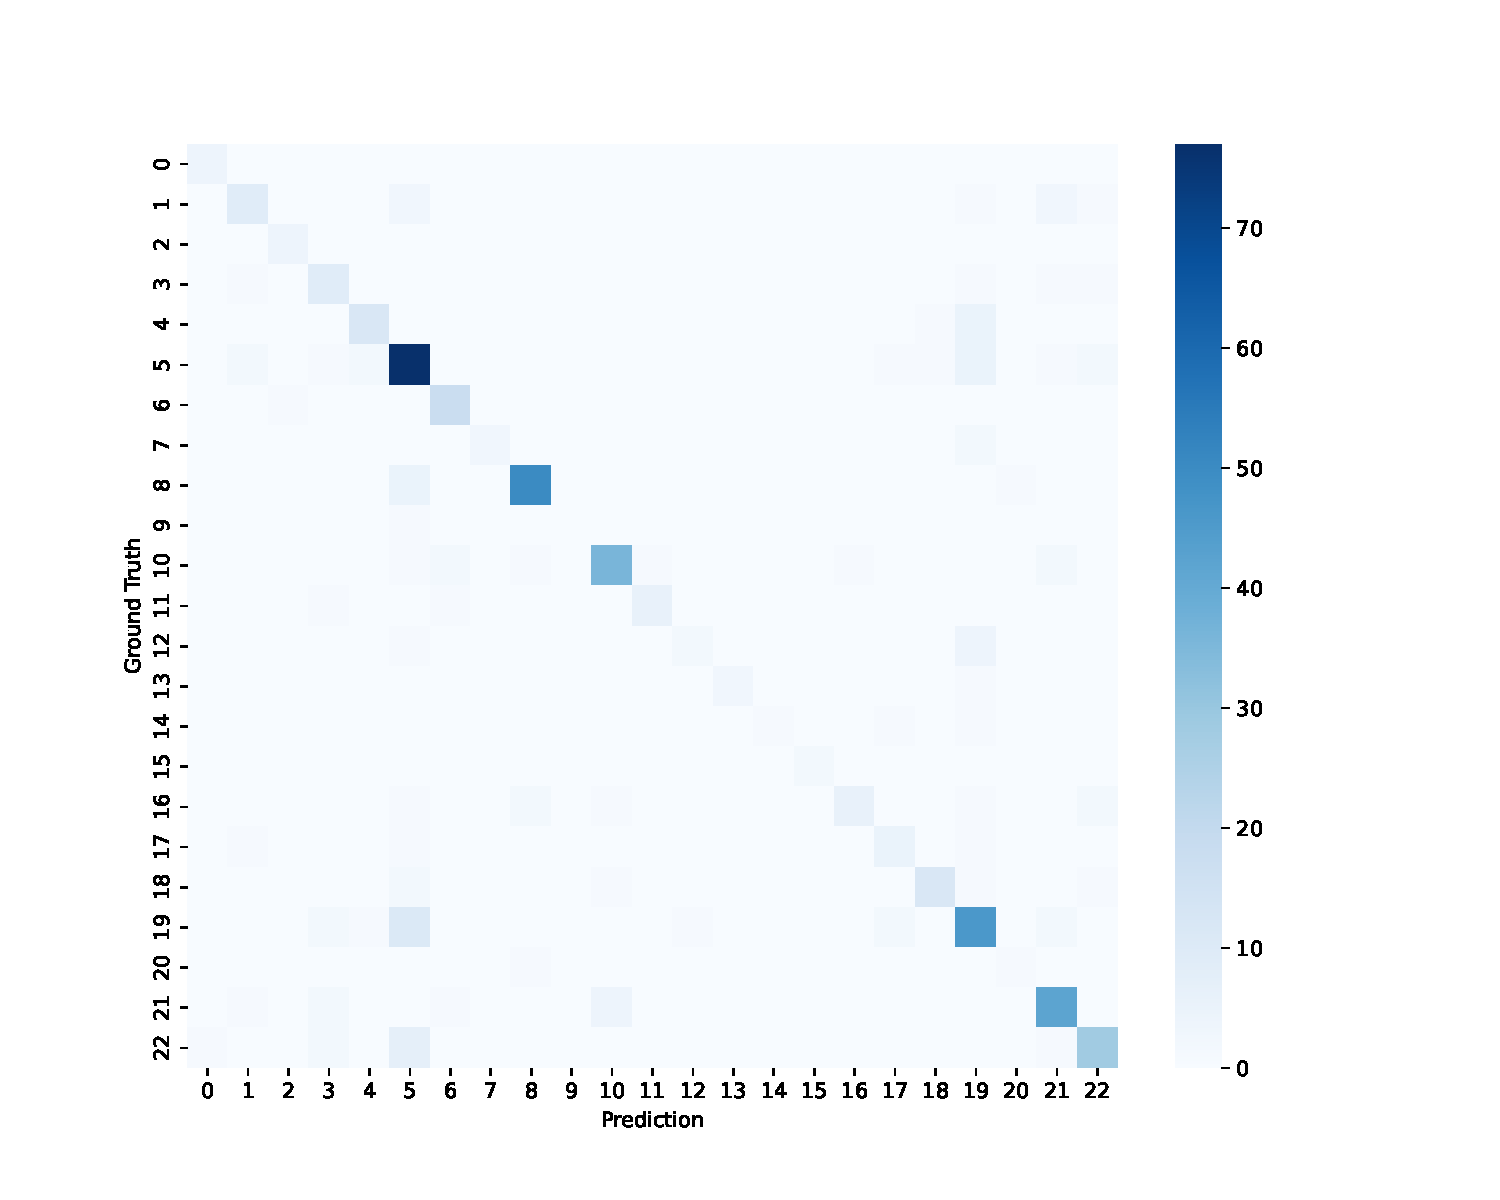
\includegraphics[width=\textwidth]{confusion_matrix_gnn.pdf}
        \caption{GCN模型}
    \end{subfigure}
    \caption{Baseline模型和GCN模型在测试集上的混淆矩阵}
    \label{tab:gcn_confusion}
\end{figure}

可以看到,GCN模型在测试集上的准确率明显高于Baseline模型。同时,相较于将许多实例错误的分类到第0类(Field Theory)的Baseline模型,GCN模型的混淆矩阵未见明显的异常。
\section{Appendix: Source Code}

\subsection{Code for Exercise 2}
\label{exercise2code}
\lstinputlisting{python_code/GP.py}






% temporarily disable the bibliography for compilation efficiency

% \bibliographystyle{plain}
% \bibliography{references}

\end{document}